\documentclass[10pt,a4paper]{article}
\usepackage[a4paper, total={7in, 11in}]{geometry}
\usepackage[utf8]{inputenc}
\usepackage{amsmath}
\usepackage{amsfonts}
\usepackage{amssymb}
\usepackage{graphicx}
\usepackage{subfig}
\author{Efeosa Eguavoen - 17324649}
\title{CSU44061 Week 2 Assignment}
\begin{document}
\maketitle
\section{A}
(i)
id:18--18-18
\begin{center}
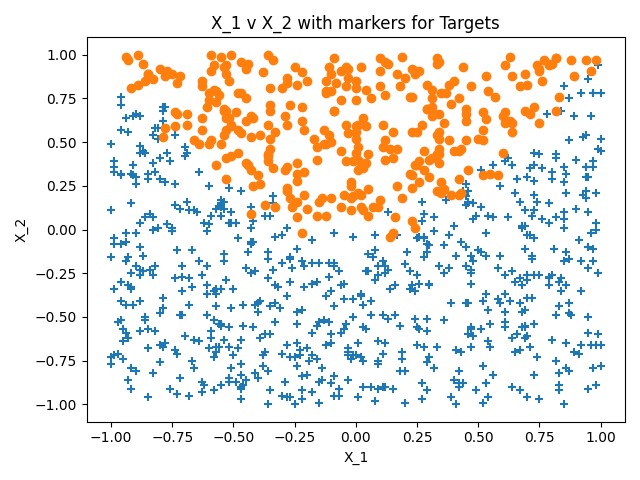
\includegraphics[scale=0.3]{x1vx2.jpg}
\end{center}
The data seems to have a sort of quadratic shape at the top with a clear distinction between the data. To derive the plot, I read in the data and placed it in a dataframe. From there I seperated the data into 2 seperate dataframes based on the value of the classification and plotted the graph with different markers for each frame. 
\begin{verbatim}
f = open("ass2.txt", "r")
start = True
data = {'x': [], 'y': [], 'z': []}
for i in f:
    if not start:
        i = i.rstrip('\n')
        vals = i.split(",")
        data['x'].append(float(vals[0]))
        data['y'].append(float(vals[1]))
        data['z'].append(int(vals[2]))
    else:
        start = False
df = pd.DataFrame(data)
df1 = df[df['z'] == -1]
df2 = df[df['z'] != -1]
\end{verbatim}
(ii)
 \(\theta_0 = -2.01562941, \theta_1 =  -0.11408452 \) \(\theta_2 =  5.85191207\)
\\
From training the model, we can see that y = +1 when \(-2.01562941 -0.11408452x_1 + 5.85191207x_2 > 0\) and y = -1 when \(< 0\)
\\
\begin{verbatim}
def loger():
    df1 = df[df['z'] == -1]
    df2 = df[df['z'] != -1]
    x = df[['x', 'y']]
    model = LogisticRegression(penalty='none', solver='lbfgs')
    model.fit(x, df['z'])
    print(model.intercept_, model.coef_)
    ys = model.predict(x)
\end{verbatim}
(iii)
\begin{center}
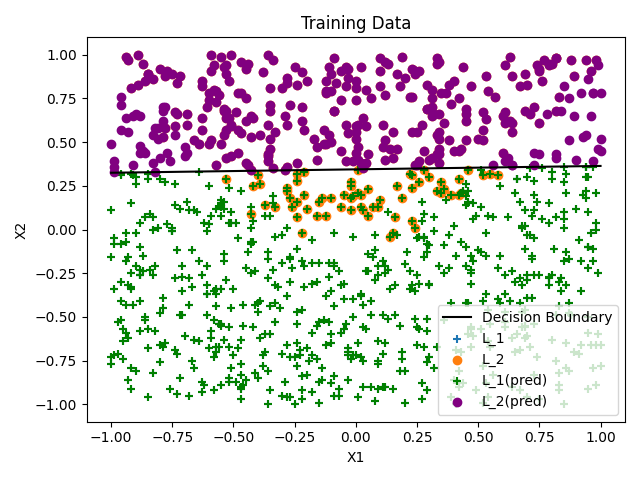
\includegraphics[scale=0.3]{x1vx2pred.jpg}
\end{center}
To obtain the decision boundary, I needed to get the correct value of \(x_2\) given \(x_1\). To achieve this, I just needed to solve the following equation: \[x_2 = -(\theta_0 + \theta_1*x_1)/\theta_2\] which gave me the correct value of y as I have the other parameters from my model. I just picked values of x between 1 and -1 using linspace and then plotted the line through those points to generate my decision boundary. I split the predictions into 2 separate dataframes to plot them also. 
\begin{verbatim}
    ys = model.predict(x)
    x['ys'] = ys
    df3 = x[x['ys'] == -1]
    df4 = x[x['ys'] != -1]

    x_vals = np.linspace(-1, 1, 50)
    y = -(model.intercept_ + model.coef_[0][0] * x_vals) / model.coef_[0][1]
\end{verbatim}
(iv)
The training data and the predictions made by the mode are accurate for the majority of cases. But as we can see in the above graph, the decision boundary is a straight line bisecting the classifications, instead of a more quadratic curve that we would expect. This causes us to have the errors in prediction like we can see towards the centre of the graph with the blue dots. Our data is clearly not linearly separable. 
\section{B}
(i)
\\ I ran values of C ranging from 0.001 to 1000, with a logarithmic scale using np.geomspace() so each value is of the same log in difference. 
\begin{verbatim}
df1 = df[df['z'] == -1]
df2 = df[df['z'] != -1]
x = df[['x', 'y']]
models = []
c_vals = np.geomspace(.001, 1000, num=7)
print(c_vals)
for i in c_vals:
        model = LinearSVC(C=i)
        model.fit(x, df['z'])
        models.append((model,i))
\end{verbatim}
The values that were reported:
\begin{table}[h]
\begin{center}
\begin{tabular}{| c | c | c | c |}
\hline
C & \(\theta_0\) & \(\theta_1\) & \(\theta_2\) \\
\hline
0.001 & -0.22455416  & -0.005645851095120078 & 0.4719346941148196 \\
\hline
0.01 & -0.22455812 & -0.00564579379445042 & 0.47193503867031295 \\
\hline
0.1 & -0.58606903 & -0.04703557261644461 & 1.7321454214013863 \\
\hline
1 & -0.64422422 & -0.04977653564180903 & 1.8907362329846127 \\
\hline
10 & -0.65199195 & -0.050029482385095074 & 1.9116600091510394 \\
\hline
100 & -0.64589482 & -0.03309475226557805 & 1.9442524392896159 \\
\hline
1000 & -0.96418217 & 0.37131381996648427 & 0.9543004068755857 \\
\hline
\end{tabular}
\caption{C values and parameters}
\end{center}
\end{table}
From the table we can see our parameters changing as our values of C change also. As our values of C change, we can see that the y intercept changes drastically, with it getting smaller as our value of C increases. 
\\
(ii)
\begin{figure}[h]
\centering
\subfloat[C = 0.001]{{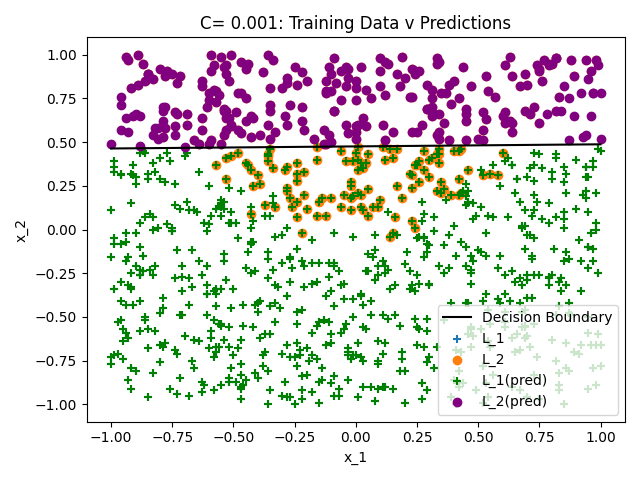
\includegraphics[width=5cm]{p1.jpg}}}
\qquad
\subfloat[C = 0.01]{{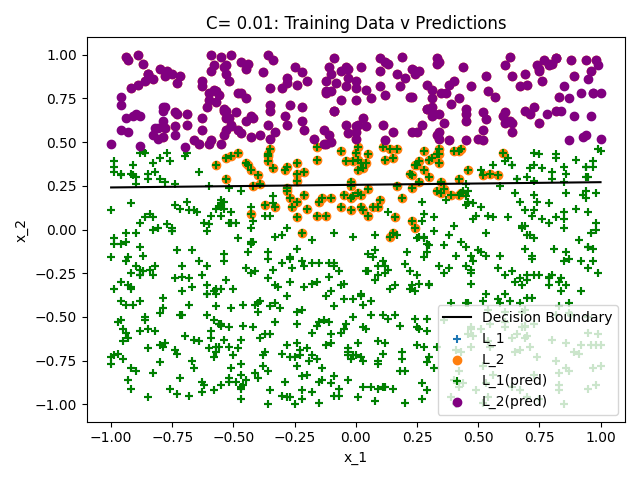
\includegraphics[width=5cm]{p2.jpg}}}
\qquad
\subfloat[C = 0.1]{{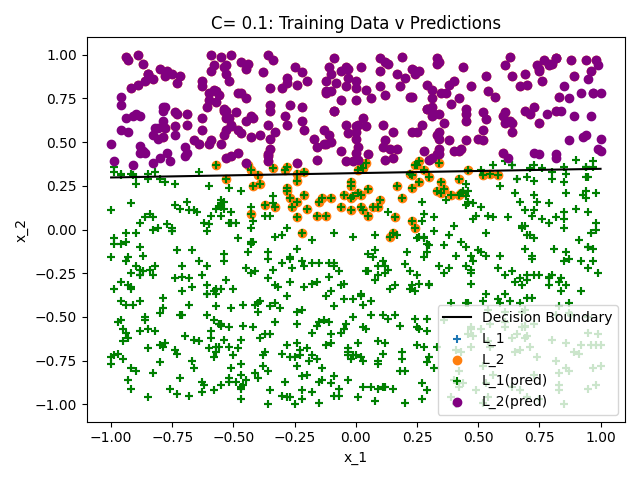
\includegraphics[width=5cm]{p3.jpg}}}
\qquad
\subfloat[C = 1]{{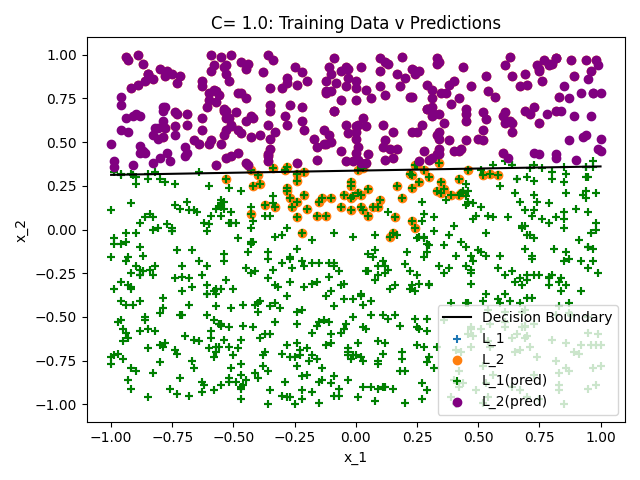
\includegraphics[width=5cm]{p4.jpg}}}
\qquad
\subfloat[C = 10]{{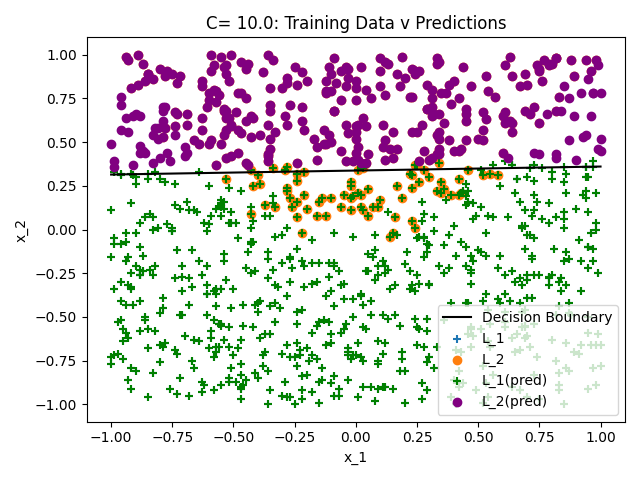
\includegraphics[width=5cm]{p5.jpg}}}
\qquad
\subfloat[C = 100]{{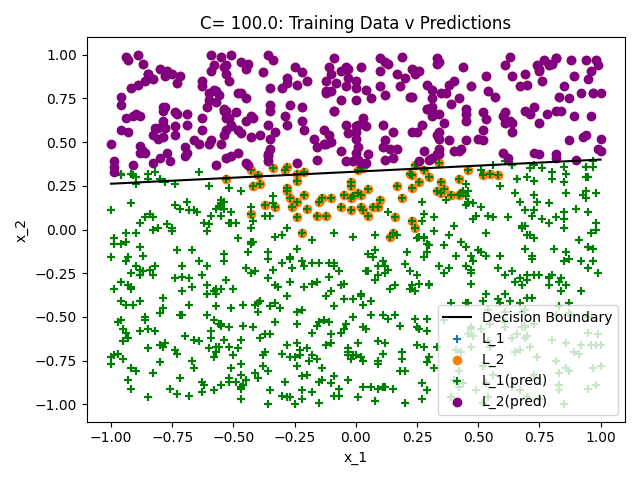
\includegraphics[width=5cm]{p6.jpg}}}
\qquad
\subfloat[C = 1000]{{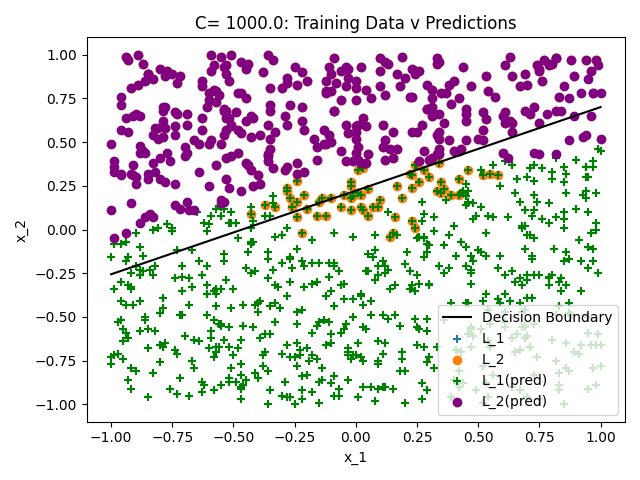
\includegraphics[width=5cm]{p7.jpg}}}
\end{figure}
To calculate the decision boundary for each of these plots, I used the same approach as I used in part A(iii). I used MatplotLib to generate all the graphs and a for loop to iterate through each of the models I had created to create each of the individual graphs.
\begin{verbatim}
    for model in models:
        plt.clf()
        model[0].fit(x,df['z'])
        ys = model[0].predict(x)
        x['ys'] = ys
        df3 = x[x['ys'] == -1]
        df4 = x[x['ys'] != -1]
        x_vals = np.linspace(-1, 1, 50)
        y = -(model[0].intercept_ + model[0].coef_[0][0] * x_vals) / model[0].coef_[0][1]
\end{verbatim}
(iii)
\\
Changing the value of C influences the decision boundary by changing the slope and the intercept of the line generated. This happens as the model attempts prevent misclassifying the data. When we've low values of C like in graph 1 and 2, we misclassified a lot of the data and we can see that with the position of the decision boundary being much higher than in the other graphs. This happens as we've got a larger margin of error so it allows for more points to be misclassified. Low values of c can even cause misclassification of linearly separable data. For larger values of C, like for C=100, we've misclassified much less of the data, and this can be seen in how the slope of the line has changed, becoming much less horizontal. But we've still got to be careful not to use too large values of C, like C = 1000 as this can make the classifier much too conservative and influences the slope a lot as it tries to prevent misclassifying any of the data.

\section{C}
(i)
To get the square of each of the features, I selected each of the individual rows with features and multiplied the value in each row by itself to get the square. I then added this as a new column in the dataframe.\\
The values reported to me by the model:  \(\theta_0 = 0.2388532  \theta_1 =-0.59851887  \) \(\theta_2 =  21.11277526 \) \( \theta_3= -26.29209894\) \(\theta_4 = 5.87851124 \). These values give me the formula for some sort of quadratic line which would match the shape of the decision boundary I would plot for the data.
\begin{verbatim}
plt.clf()
    df['x3'] = df['x']**2
    df['x4'] = df['y']**2
    df1 = df[df['z'] == -1]
    df2 = df[df['z'] != -1]
    x = df[['x', 'y']]
    square = df[['x', 'y', 'x3', 'x4']]
    model = LogisticRegression(penalty='none', solver='lbfgs')
    model.fit(square, df['z'])
    print(model.intercept_, model.coef_)
\end{verbatim}
(ii)
\begin{figure}[h]
\centering
\subfloat[Training vs Predictions]{{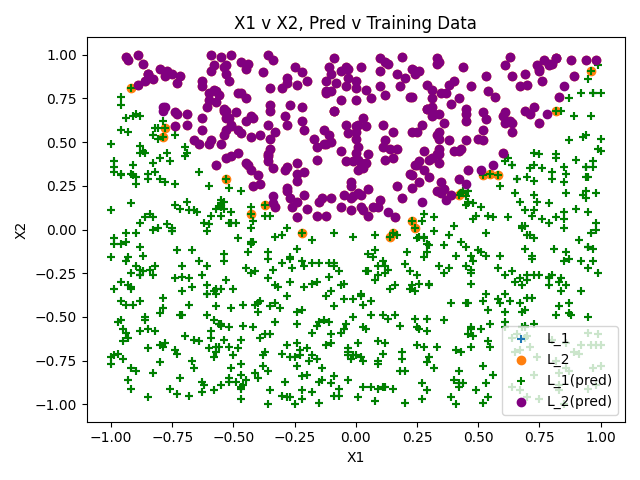
\includegraphics[scale=0.3]{sqr.jpg}}}
\qquad
\subfloat[Training data]{{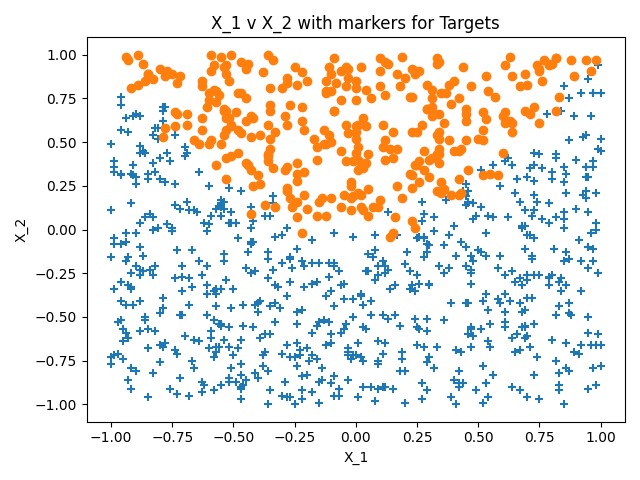
\includegraphics[scale=0.3]{x1vx2.jpg}}}
\end{figure}
When we add the squared features to the dataset and add this data to our model, we can see our predictions become much more accurate for each classification of data. The decision boundary would be quadratic in shape roughly, so squaring the features gives us a quadratic model also. While the model isn't perfect, overall it fits the data much more accurately than our linear model. 
\begin{verbatim}
ys = model.predict(square)
    x['ys'] = ys
    df3 = x[x['ys'] == -1]
    df4 = x[x['ys'] != -1]
\end{verbatim}
(iii)
For the baseline model, I used a predictor based of the ratio of the data. From the data I could see it's split roughly 70/30 so I let it predict one class 70\(\%\) of the time and the other the rest of the time. I generated 999 numbers between 1 and 10 from there turned those numbers into a +1 or -1 depending on if it was bigger than 7 or not. I then appended the results to the dataframe.
\\
From this, I then put the number of correct predictions over the number of points. I did this multiple times to get an average. On average, using this method, I got the correct class 58\(\%\) of the time giving me an accuracy of 58\(\%\). In comparison, using the model, I got the correct class 97\(\%\) of the time.
\\
Using the random model as my baseline, I could see that the model I created using Logistic regression was significantly better than the baseline model I created. While I expected the random model to be more accurate than it is, due to the fact it's generating a random number between 1 and 10 for it to be classified is probably why there's a higher error rate than just guessing the most prevalent class in the dataset.
\begin{verbatim}
v = np.random.randint(10,size=999)
    for i in range(len(v)):
        if v[i] >= 7:
            v[i] = -1
        else:
            v[i] = -1
    df['rand'] = v
    df5 = df[df['rand'] == -1]
    df6 = df[df['rand'] != -1]
    num = df[df['rand'] == df['z']]
    num2 = df[df['z'] == ys]
    print(len(num), len(num2))
\end{verbatim}


\section{Appendix: Code}
\begin{verbatim}
import pandas as pd
import matplotlib.pyplot as plt
import numpy as np
from sklearn.linear_model import LogisticRegression
from sklearn.svm import LinearSVC

f = open("ass2.txt", "r")
start = True
data = {'x': [], 'y': [], 'z': []}
for i in f:
    if not start:
        i = i.rstrip('\n')
        vals = i.split(",")
        data['x'].append(float(vals[0]))
        data['y'].append(float(vals[1]))
        data['z'].append(int(vals[2]))
    else:
        start = False
df = pd.DataFrame(data)



def loger():
    df1 = df[df['z'] == -1]
    df2 = df[df['z'] != -1]
    x = df[['x', 'y']]
    model = LogisticRegression(penalty='none', solver='lbfgs')
    model.fit(x, df['z'])
    print(model.intercept_, model.coef_)
    ys = model.predict(x)
    x['ys'] = ys
    df3 = x[x['ys'] == -1]
    df4 = x[x['ys'] != -1]

    x_vals = np.linspace(-1, 1, 50)
    y = -(model.intercept_ + model.coef_[0][0] * x_vals) / model.coef_[0][1]
    plt.scatter(df1['x'], df1['y'], marker='+')
    plt.scatter(df2['x'], df2['y'], marker='o')
    plt.scatter(df3['x'], df3['y'], marker='+', color='green')
    plt.scatter(df4['x'], df4['y'], marker='o', color='purple')
    plt.plot(x_vals,y, color='black')
    plt.legend(["Decision Boundary","L_1", "L_2", "L_1(pred)", "L_2(pred)"])
    plt.title(f"Training Data")
    plt.xlabel('X1')
    plt.ylabel('X2')
    plt.show()


def svm():
    df1 = df[df['z'] == -1]
    df2 = df[df['z'] != -1]
    x = df[['x', 'y']]
    models = []
    c_vals = np.geomspace(.001, 1000, num=7)
    print(c_vals)
    for i in c_vals:
        model = LinearSVC(C=i)
        model.fit(x, df['z'])
        models.append((model,i))

    for model in models:
        plt.clf()
        model[0].fit(x,df['z'])
        ys = model[0].predict(x)
        x['ys'] = ys
        df3 = x[x['ys'] == -1]
        df4 = x[x['ys'] != -1]
        x_vals = np.linspace(-1, 1, 50)
        y = -(model[0].intercept_ + model[0].coef_[0][0] * x_vals) / model[0].coef_[0][1]
        plt.scatter(df1['x'], df1['y'], marker='+')
        plt.scatter(df2['x'], df2['y'], marker='o')
        plt.scatter(df3['x'], df3['y'], marker='+', color='green')
        plt.scatter(df4['x'], df4['y'], marker='o', color='purple')
        plt.plot(x_vals, y, color='black')
        plt.legend(["Decision Boundary", "L_1", "L_2", "L_1(pred)", "L_2(pred)" ])
        plt.title(f"C= {model[1]}: Training Data v Predictions")
        plt.xlabel("x_1")
        plt.ylabel("x_2")
        plt.show()
        plt.clf()

def squared():
    plt.clf()
    df['x3'] = df['x']**2
    df['x4'] = df['y']**2
    df1 = df[df['z'] == -1]
    df2 = df[df['z'] != -1]
    x = df[['x', 'y']]
    square = df[['x', 'y', 'x3', 'x4']]
    model = LogisticRegression(penalty='none', solver='lbfgs')
    model.fit(square, df['z'])
    print(model.intercept_, model.coef_)
    ys = model.predict(square)
    x['ys'] = ys
    df3 = x[x['ys'] == -1]
    df4 = x[x['ys'] != -1]
    plt.scatter(df1['x'], df1['y'], marker='+')
    plt.scatter(df2['x'], df2['y'], marker='o')
    plt.scatter(df3['x'], df3['y'], marker='+', color='green')
    plt.scatter(df4['x'], df4['y'], marker='o', color='purple')
    plt.legend(["L_1", "L_2", "L_1(pred)", "L_2(pred)"])
    plt.title(f"X1 v X2, Pred v Training Data")
    plt.xlabel('X1')
    plt.ylabel('X2')
    plt.show()

    v = np.random.randint(10,size=999)
    for i in range(len(v)):
        if v[i] >= 7:
            v[i] = -1
        else:
            v[i] = -1
    df['rand'] = v
    df5 = df[df['rand'] == -1]
    df6 = df[df['rand'] != -1]
    plt.clf()
    plt.scatter(df1['x'], df1['y'], marker='+')
    plt.scatter(df2['x'], df2['y'], marker='o')
    plt.scatter(df5['x'], df5['y'], marker='+', color='green')
    plt.scatter(df6['x'], df6['y'], marker='o', color='purple')
    plt.show()
    num = df[df['rand'] == df['z']]
    num2 = df[df['z'] == ys]
    print(len(num), len(num2))

\end{verbatim}
\end{document}